\documentclass[onlymath]{beamer}
% \documentclass[onlymath,handout]{beamer}

% Macros used by all lectures, but not necessarily by excercises

%%% General setup and dependencies:

% \usetheme[ddcfooter,nosectionnum]{tud}
\usetheme[nosectionnum,pagenum,noheader]{tud}
% \usetheme[nosectionnum,pagenum]{tud}

% Increase body font size to a sane level:
\let\origframetitle\frametitle
% \renewcommand{\frametitle}[1]{\origframetitle{#1}\normalsize}
\renewcommand{\frametitle}[1]{\origframetitle{#1}\fontsize{10pt}{13.2}\selectfont}
\setbeamerfont{itemize/enumerate subbody}{size=\small} % tud defaults to scriptsize!
\setbeamerfont{itemize/enumerate subsubbody}{size=\small}
% \setbeamerfont{normal text}{size=\small}
% \setbeamerfont{itemize body}{size=\small}

\renewcommand{\emph}[1]{\textbf{#1}}

\def\arraystretch{1.3}% Make tables even less cramped vertically

\usepackage[ngerman]{babel}
\usepackage[utf8]{inputenc}
\usepackage[T1]{fontenc}

%\usepackage{graphicx}
\usepackage[export]{adjustbox} % loads graphicx
\usepackage{import}
\usepackage{stmaryrd}
\usepackage[normalem]{ulem} % sout command
% \usepackage{times}
\usepackage{txfonts}
\usepackage{array}

% \usepackage[perpage]{footmisc} % reset footnote counter on each page -- fails with beamer (footnotes gone)
\usepackage{perpage}  % reset footnote counter on each page
\MakePerPage{footnote}

\usepackage{tikz}
\usetikzlibrary{arrows,positioning,decorations.pathreplacing}
% Inspired by http://www.texample.net/tikz/examples/hand-drawn-lines/
\usetikzlibrary{decorations.pathmorphing}
\pgfdeclaredecoration{penciline}{initial}{
    \state{initial}[width=+\pgfdecoratedinputsegmentremainingdistance,
    auto corner on length=1mm,]{
        \pgfpathcurveto%
        {% From
            \pgfqpoint{\pgfdecoratedinputsegmentremainingdistance}
                      {\pgfdecorationsegmentamplitude}
        }
        {%  Control 1
        \pgfmathrand
        \pgfpointadd{\pgfqpoint{\pgfdecoratedinputsegmentremainingdistance}{0pt}}
                    {\pgfqpoint{-\pgfdecorationsegmentaspect
                     \pgfdecoratedinputsegmentremainingdistance}%
                               {\pgfmathresult\pgfdecorationsegmentamplitude}
                    }
        }
        {%TO
        \pgfpointadd{\pgfpointdecoratedinputsegmentlast}{\pgfpoint{1pt}{1pt}}
        }
    }
    \state{final}{}
}
\tikzset{handdrawn/.style={decorate,decoration=penciline}}
\tikzset{every shadow/.style={fill=none,shadow xshift=0pt,shadow yshift=0pt}}
% \tikzset{module/.append style={top color=\col,bottom color=\col}}

% Use to make Tikz attributes with Beamer overlays
% http://tex.stackexchange.com/a/6155
\tikzset{onslide/.code args={<#1>#2}{%
  \only<#1| handout:0>{\pgfkeysalso{#2}}
}}
\tikzset{onslideprint/.code args={<#1>#2}{%
  \only<#1>{\pgfkeysalso{#2}}
}}

%%% Title -- always set this first

\newcommand{\defineTitle}[3]{
	\newcommand{\lectureindex}{#1}
	\title{Theoretische Informatik und Logik}
	\subtitle{\href{\lectureurl}{#1. Vorlesung: #2}}
	\author{\href{https://iccl.inf.tu-dresden.de/web/Markus_Kr\%C3\%B6tzsch}{Markus Kr\"{o}tzsch}\\[1ex]Lehrstuhl Wissensbasierte Systeme}
	\date{#3}
	\datecity{TU Dresden}
% 	\institute{CC-By 3.0, sofern keine anderslautenden Bildrechte angegeben sind}
}

%%% Table of contents:

\RequirePackage{ifthen}

\newcommand{\highlight}[2]{%
	\ifthenelse{\equal{#1}{\lectureindex}}{\alert{#2}}{#2}%
}

\def\myspace{-0.7ex}
\newcommand{\printtoc}{
\begin{tabular}{r@{$\quad$}l}
\highlight{1}{1.} & \highlight{1}{Willkommen/Einleitung formale Sprachen}\\[\myspace]
\highlight{2}{2.} & \highlight{2}{Grammatiken und die Chomsky-Hierarchie}\\[\myspace]
\highlight{3}{3.} & \highlight{3}{Endliche Automaten}\\[\myspace]
\highlight{4}{4.} & \highlight{4}{Complexity of FO query answering}\\[\myspace]
\highlight{5}{5.} & \highlight{5}{Conjunctive queries}\\[\myspace]
\highlight{6}{6.} & \highlight{6}{Tree-like conjunctive queries}\\[\myspace]
\highlight{7}{7.} & \highlight{7}{Query optimisation}\\[\myspace]
\highlight{8}{8.} & \highlight{8}{Conjunctive Query Optimisation / First-Order~Expressiveness}\\[\myspace]
\highlight{9}{9.} & \highlight{9}{First-Order~Expressiveness / Introduction to Datalog}\\[\myspace]
\highlight{10}{10.} & \highlight{10}{Expressive Power and Complexity of Datalog}\\[\myspace]
\highlight{11}{11.} & \highlight{11}{Optimisation and Evaluation of Datalog}\\[\myspace]
\highlight{12}{12.} & \highlight{12}{Evaluation of Datalog (2)}\\[\myspace]
\highlight{13}{13.} & \highlight{13}{Graph Databases and Path Queries}\\[\myspace]
\highlight{14}{14.} & \highlight{14}{Outlook: database theory in practice}
\end{tabular}
}

\newcommand{\overviewslide}{%
\begin{frame}\frametitle{Overview}
\printtoc
\medskip

Siehe \href{\lectureurl}{course homepage [$\Rightarrow$ link]} for more information and materials
\end{frame}
}

%%% Colours:
\usepackage{xcolor,colortbl}
\definecolor{redhighlights}{HTML}{FFAA66}
\definecolor{lightblue}{HTML}{55AAFF}
\definecolor{lightred}{HTML}{FF5522}
\definecolor{lightpurple}{HTML}{DD77BB}
\definecolor{lightgreen}{HTML}{55FF55}
\definecolor{darkred}{HTML}{CC4411}
\definecolor{darkblue}{HTML}{176FC0}%{1133AA}
\definecolor{nightblue}{HTML}{2010A0}%{1133AA}
\definecolor{alert}{HTML}{176FC0}
\definecolor{darkgreen}{HTML}{36AB14}
\definecolor{strongyellow}{HTML}{FFE219}
\definecolor{devilscss}{HTML}{666666}

\newcommand{\redalert}[1]{\textcolor{darkred}{#1}}

%%% Slide layout commands:

\newcommand{\sectionSlide}[1]{
\frame{\begin{center}
\LARGE
#1
\end{center}}
}
\newcommand{\sectionSlideNoHandout}[1]{
\frame<handout:0>{\begin{center}
\LARGE
#1
\end{center}}
}

\newcommand{\mydualbox}[3]{%
 \begin{minipage}[t]{#1}
 \begin{beamerboxesrounded}[upper=block title,lower=block body,shadow=true]%
    {\centering\usebeamerfont*{block title}#2}%
    \raggedright%
    \usebeamerfont{block body}
%     \small
    #3%
  \end{beamerboxesrounded}
  \end{minipage}
}
%
\newcommand{\myheaderbox}[2]{%
 \begin{minipage}[t]{#1}
 \begin{beamerboxesrounded}[upper=block title,lower=block title,shadow=true]%
    {\centering\usebeamerfont*{block title}\rule{0pt}{2.6ex} #2}%
  \end{beamerboxesrounded}
  \end{minipage}
}

\newcommand{\mycontentbox}[2]{%
 \begin{minipage}[t]{#1}%
 \begin{beamerboxesrounded}[upper=block body,lower=block body,shadow=true]%
    {\centering\usebeamerfont*{block body}\rule{0pt}{2.6ex}#2}%
  \end{beamerboxesrounded}
  \end{minipage}
}

\newcommand{\mylcontentbox}[2]{%
 \begin{minipage}[t]{#1}%
 \begin{beamerboxesrounded}[upper=block body,lower=block body,shadow=true]%
    {\flushleft\usebeamerfont*{block body}\rule{0pt}{2.6ex}#2}%
  \end{beamerboxesrounded}
  \end{minipage}
}

% label=180:{\rotatebox{90}{{\footnotesize\textcolor{darkgreen}{Beispiel}}}}
% \hspace{-8mm}\ghost{\raisebox{-7mm}{\rotatebox{90}{{\footnotesize\textcolor{darkgreen}{Beispiel}}}}}\hspace{8mm}
\newcommand{\examplebox}[1]{%
	\begin{tikzpicture}[decoration=penciline, decorate]
		\pgfmathsetseed{1235}
		\node (n1) [decorate,draw=darkgreen, fill=darkgreen!10,thick,align=left,text width=\linewidth, inner ysep=2mm, inner xsep=2mm] at (0,0) {#1};
% 		\node (n2) [align=left,text width=\linewidth,inner sep=0mm] at (n1.92) {{\footnotesize\raisebox{3mm}{\textcolor{darkgreen}{Beispiel}}}};
% 		\node (n2) [decorate,draw=darkgreen, fill=darkgreen!10,thick, align=left,text width=\linewidth,inner sep=2mm] at (n1.90) {{\footnotesize\raisebox{0mm}{\textcolor{darkgreen}{Beispiel}}}};
	\end{tikzpicture}%
}%

\newcommand{\codebox}[1]{%
	\begin{tikzpicture}[decoration=penciline, decorate]
		\pgfmathsetseed{1236}
		\node (n1) [decorate,draw=strongyellow, fill=strongyellow!10,thick,align=left,text width=\linewidth, inner ysep=2mm, inner xsep=2mm] at (0,0) {#1};
	\end{tikzpicture}%
}%

\newcommand{\defbox}[1]{%
	\begin{tikzpicture}[decoration=penciline, decorate]
		\pgfmathsetseed{1237}
		\node (n1) [decorate,draw=darkred, fill=darkred!10,thick,align=left,text width=\linewidth, inner ysep=2mm, inner xsep=2mm] at (0,0) {#1};
	\end{tikzpicture}%
}%

\newcommand{\theobox}[1]{%
	\begin{tikzpicture}[decoration=penciline, decorate]
		\pgfmathsetseed{1240}
		\node (n1) [decorate,draw=darkblue, fill=darkblue!10,thick,align=left,text width=\linewidth, inner ysep=2mm, inner xsep=2mm] at (0,0) {#1};
	\end{tikzpicture}%
}%

\newcommand{\anybox}[2]{%
	\begin{tikzpicture}[decoration=penciline, decorate]
		\pgfmathsetseed{1240}
		\node (n1) [decorate,draw=#1, fill=#1!10,thick,align=left,text width=\linewidth, inner ysep=2mm, inner xsep=2mm] at (0,0) {#2};
	\end{tikzpicture}%
}%


\newsavebox{\mybox}%
\newcommand{\doodlebox}[2]{%
\sbox{\mybox}{#2}%
	\begin{tikzpicture}[decoration=penciline, decorate]
		\pgfmathsetseed{1238}
		\node (n1) [decorate,draw=#1, fill=#1!10,thick,align=left,inner sep=1mm] at (0,0) {\usebox{\mybox}};
	\end{tikzpicture}%
}%


\defineTitle{15}{Logisches Schließen}{14. Juni 2017}

\begin{document}

\maketitle

\begin{frame}\frametitle{Ankündigung}

\begin{center}
Prüfungstermin im Sommersemester 2017:\\[3ex]

{\huge 24. Juli 2017}\\[3ex]

Lernräume werden organisiert und auf der Webseite angekündigt.
\end{center}

\end{frame}

\begin{frame}\label{frame_logiker}\frametitle{Prädikatenlogik als Universalsprache}

Die Entwicklung der Logik hat ein zentrales Motiv:\\
\alert{Logik als eine universelle, präzise Sprache}\pause

\begin{itemize}
\item \ghost{\hspace{-1.5cm}\raisebox{-11mm}{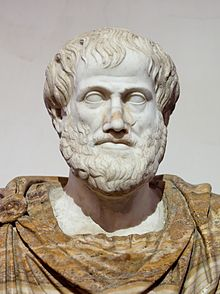
\includegraphics[width=1cm]{images/Aristotle}}}%
	Aristoteles (384--322 v.Chr.): Logik als Grundlage der (philosophischen) Argumentation zwischen vernünftig denkenden Menschen\pause
\item \ghost{\hspace{-1.5cm}\raisebox{-13.5mm}{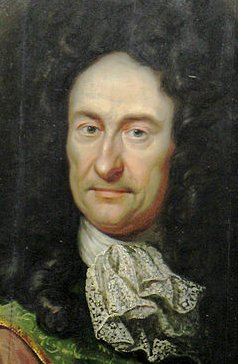
\includegraphics[width=1cm]{images/Leibniz}}}%
	Leibniz (1646--1716): Vordenker des automatischen \ghost{Schließens:}\\
\anybox{purple}{{\footnotesize
"`\ldots falls es zu Unstimmigkeiten käme, dann gäbe es zwischen zwei Philosophen nicht mehr Anlass für Streitigkeiten als zwischen zwei Buchhaltern. Denn es würde genügen, dass beide die Stifte zur Hand nehmen, sich zum Rechenschieber setzen und sagen \ghost{[{\scalebox{0.8}{$\cdots$\hspace{-1pt}}}]:}\\ \alert{Lasst uns rechnen!}"'

}}\pause
\item \ghost{\hspace{-1.5cm}\raisebox{0.5mm}{\includegraphics[width=1cm]{images/Hilbert}}}%
	Hilbert (1862--1942): Programm zur Formalisierung der Mathematik\pause
\item \ghost{\hspace{-1.5cm}\raisebox{-5mm}{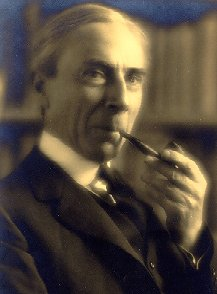
\includegraphics[width=1cm]{images/Russell}}}%
	Russell (1872--1970): Entwicklung eines logischen Kalküls als Grundlage aller Mathematik
\end{itemize}

\end{frame}

\begin{frame}\frametitle{Kernproblem logisches Schließen}

Drückt man die Mathematik in logischen Formeln aus, dann wird\\
logisches Schließen zur Kernaufgabe mathematischer Forschung\bigskip

\defbox{Das Problem des prädikatenlogischen Schließens besteht in der folgenden Frage:\\[1ex]
\emph{Gegeben:} Eine endliche Menge prädikatenlogischer Sätze (Theorie) $\mathcal{T}$ und ein Satz $F$\\
\emph{Frage:} Gilt $\mathcal{T}\models F$, d.h. folgt $F$ aus $\mathcal{T}$?
}\pause

Dieses Problem ist zu verschiedenen anderen äquivalent:

\theobox{Satz: Für endliche Theorie $\mathcal{T}$ und einen Satz $F$ sind die folgenden Fragen äquivalent:
\begin{itemize}
\item Gilt $\mathcal{T}\models F$?
\item Ist $\mathcal{T}\cup \{\neg F\}$ unerfüllbar? 
\item Ist $\bigwedge_{G\in\mathcal{T}} G\to F$ eine Tautologie? 
\end{itemize}
}

\end{frame}

\begin{frame}\frametitle{Die Bedeutung von Erfüllbarkeit}

\theobox{Satz: Für endliche Theorie $\mathcal{T}$ und einen Satz $F$ sind die folgenden Fragen äquivalent:
\begin{itemize}
\item Gilt $\mathcal{T}\models F$?
\item Ist $\mathcal{T}\cup \{\neg F\}$ unerfüllbar? 
\item Ist $\bigwedge_{G\in\mathcal{T}} G\to F$ eine Tautologie? 
\end{itemize}
}

\emph{Daraus folgt:} Logisches Schließen kann auf das Überprüfen der Erfüllbarkeit einer Formel
\[ \bigwedge_{G\in\mathcal{T}}G\wedge \neg F \]
zurückgeführt werden\bigskip

\redalert{$\leadsto$ Erfüllbarkeit als zentrale Frage des Schließens}

\end{frame}

\sectionSlide{Gleichheit}

\begin{frame}\frametitle{Gleichheit in Prädikatenlogik}

Gleichheit spielt in vielen Anwendungen eine große Rolle:\smallskip

Manchmal wird Prädikatenlogik so definiert, dass es ein
spezielles \redalert{Gleichheitsprädikat $\approx$} gibt, welches man in der Regel infix schreibt
\bigskip

\emph{Semantik:} In allen Interpretationen $\Inter$ ist $\approx^\Inter=\{\tuple{\delta,\delta}\mid \delta\in\Delta^\Inter\}$.
\bigskip\pause

Wir haben bereits ein Beispiel dafür gesehen:

\examplebox{Beispiel: Partielle Ordnungen $\preceq$ sind antisymmetrisch:\vspace{-0.5ex}
\begin{align*}
\forall x,y. & \big(( x\preceq y \wedge y\preceq x )\to x\approx y\big)
\end{align*}\vspace{-3ex}
}\pause

Auch erlaubt uns Gleichheit, in Logik zu zählen:

\examplebox{Beispiel: "`Es gibt nur einen Rudi Völler"' (erster Suchvorschlag von Google bei Eingabe "`Es gibt nur einen "', Stand Mai 2017)
\begin{align*}
\forall x,y.\big(\textsf{rudiVöller}(x)\wedge \textsf{rudiVöller}(y)\to x\approx y\big)
\end{align*}
}

% \emph{Zusatzaufgabe:} Formalisieren Sie "`Es gibt "'

\end{frame}

\begin{frame}\frametitle{Gleichheit der Interpretation von Konstanten}

Die übliche Semantik von Prädikatenlogik erlaubt, dass verschiedene 
Konstanten gleich interpretiert werden.\bigskip

Mit Gleichheit kann man das erzwingen oder verbieten:
\examplebox{Beispiel: Seien nun $\textsf{rudiVöller},\textsf{tanteKäthe},\textsf{rudi}\in\Slang{C}$ Konstanten. Wir können ausdrücken:
\begin{align*}
\textsf{rudiVöller}&\approx\textsf{tanteKäthe}\\
\neg\; \textsf{rudiVöller}&\approx\textsf{rudi}\\
\end{align*}\vspace{-8ex}

~
}

Manchmal wird auch $\not\approx$ als spezielles Prädikat eingeführt.\\
Wir können das aber auch leicht definieren:
\[ \forall x,y.(x\not\approx y\leftrightarrow \neg x\approx y)\]

\end{frame}

\newcommand{\eqpred}{\textsf{eq}}

\begin{frame}\frametitle{Ist Ungleichheit wirklich nötig?}

Ungleichheit von Konstanten kann man auch leicht ohne $\approx$ ausdrücken:\medskip

\examplebox{Beispiel: Wir betrachten zwei neue, einstellige Prädikate $O_{\textsf{rudiVöller}}$ und $O_{\textsf{rudi}}$. Die folgende Theorie
impliziert $\neg \textsf{rudiVöller}\approx\textsf{rudi}$:
\begin{align*}
O_{\textsf{rudiVöller}}(\textsf{rudiVöller})  & & O_{\textsf{rudi}}(\textsf{rudi}) &&
\forall x. \neg (O_{\textsf{rudiVöller}}(x)\wedge O_{\textsf{rudi}}(x))
\end{align*}
}\pause

\emph{Idee:}
\begin{itemize}
\item Die Prädikate $O_{\textsf{rudiVöller}}$ und $O_{\textsf{rudi}}$ beschreiben zwei Mengen
\item Die Mengen enthalten jeweils mindestens die Elemente, welche durch $\textsf{rudiVöller}$ bzw. $\textsf{rudi}$ bezeichnet werden
\item Die Mengen sind disjunkt (d.h. enthalten keine gemeinsamen Elemente)
\end{itemize}
\redalert{$\leadsto$ Erzwingung von Ungleichheit durch Zuweisung unvereinbarer Eigenschaften}

\end{frame}

\begin{frame}\frametitle{Ist Gleichheit wirklich nötig?}

Es stellt sich heraus, dass man die wesentlichen Eigenschaften von $\approx$ logisch beschreiben kann:

\defbox{Für eine gegebene endliche Menge $\Slang{R}$ von relevanten Prädikatensymbolen
und ein neues zweistelliges Prädikatensymbol $\eqpred$ definieren wir
die folgende \redalert{Gleichheitstheorie} $\mathcal{EQ}_{\Slang{R}}$:
\begin{align*}
\forall x.&\eqpred(x,x) & \text{Reflexivität} \\
\forall x,y.&\eqpred(x,y)\to\eqpred(y,x) & \text{Symmetrie}\\
\forall x,y,z.&\eqpred(x,y)\wedge\eqpred(y,z)\to\eqpred(x,z) & \text{Transitivität}\\
\forall x_1,\ldots,x_n,y. & \big((p(x_1,\ldots, x_{i-1},\alert{x_i},x_{i+1},\ldots,x_n)\wedge\eqpred(\alert{x_i},\alert{y}) )\\
&\hspace{1.3cm}\to p(x_1,\ldots, x_{i-1},\alert{y},x_{i+1},\ldots,x_n)\big) & \text{Kongruenz}
\end{align*}
wobei der letzte Satz für alle $n$-stelligen $p\in\Slang{R}$ und alle $i\in\{1,\ldots,n\}$
instanziiert wird ($\leadsto$ endlich viele Sätze).
}

\end{frame}

\begin{frame}\frametitle{Gleichheit ist nicht nötig}

Für eine beliebige Theorie $\mathcal{T}$ der Prädikatenlogik mit Gleichheit
definieren wir \redalert{$\mathcal{T}_{\eqpred}$} als die Theorie, die man erhält,
indem man $\approx$ in allen Sätzen von $\mathcal{T}$ durch $\eqpred$ ersetzt.
\bigskip

\theobox{Satz: Sei $\mathcal{T}$ eine Theorie der Prädikatenlogik mit $\approx$
und weiteren Prädikatensymbolen aus der endlichen Menge $\Slang{R}$.\medskip

Dann ist $\mathcal{T}$ genau dann in der Prädikatenlogik mit Gleichheit erfüllbar wenn $\mathcal{T}_{\eqpred}\cup\mathcal{EQ}_{\Slang{R}}$ in der Prädikatenlogik ohne Gleichheit erfüllbar ist.
}\pause

\emph{Warum ist das nützlich?}
\begin{itemize}
\item Logisches Schließen kann auf den Test von Erfüllbarkeit zurückgeführt werden
\item Erfüllbarkeit bleibt erhalten, wenn man "`eingebaute"' Gleicheit durch eine logische 
Beschreibung von Gleichheit ersetzt
\end{itemize}
\redalert{$\leadsto$ Schließen wird durch Gleichheit nicht wesentlich komplizierter}

\end{frame}

\begin{frame}[t]\frametitle{Beweis (1)}

\theobox{Satz: Sei $\mathcal{T}$ eine Theorie der Prädikatenlogik mit $\approx$
und weiteren Prädikatensymbolen aus der endlichen Menge $\Slang{R}$.\medskip

Dann ist $\mathcal{T}$ genau dann in der Prädikatenlogik mit Gleichheit erfüllbar wenn $\mathcal{T}_{\eqpred}\cup\mathcal{EQ}_{\Slang{R}}$ in der Prädikatenlogik ohne Gleichheit erfüllbar ist.
}

\emph{Beweis:} "`$\Rightarrow$"' Nehmen wir an, $\mathcal{T}$ ist in der Prädikatenlogik mit Gleichheit erfüllbar.\pause
\begin{itemize}
\item Dann hat $\mathcal{T}$ ein Modell $\Inter\models\mathcal{T}$, wobei $\approx^\Inter=\{\tuple{\delta,\delta}\mid \delta\in\Delta^\Inter\}$\pause
\item Wir definieren eine Interpretation $\Jnter$ mit $\Delta^\Jnter\defeq\Delta^\Inter$:
	\begin{itemize}
	\item $c^\Jnter\defeq c^\Inter$ für alle Konstanten $c\in\Slang{C}$
	\item $p^\Jnter\defeq p^\Inter$ für alle Prädikate $p\in\Slang{P}$ mit $p\neq{\approx}$
	\item $\eqpred^\Jnter\defeq {\approx^\Inter}$
	\end{itemize}\pause
\item Dann gilt $\Jnter\models\mathcal{T}_{\eqpred}$ per Definition\pause
\item Zudem gilt $\Jnter\models\mathcal{EQ}_{\Slang{R}}$, da $\eqpred^\Jnter=\{\tuple{\delta,\delta}\mid \delta\in\Delta^\Jnter\}$\pause
\end{itemize}
$\leadsto$ $\Jnter\models\mathcal{T}_{\eqpred}\cup\mathcal{EQ}_{\Slang{R}}$, das heißt $\mathcal{T}_{\eqpred}\cup\mathcal{EQ}_{\Slang{R}}$ ist erfüllbar
\end{frame}

\begin{frame}[t]\frametitle{Beweis (2)}

\theobox{Satz: Sei $\mathcal{T}$ eine Theorie der Prädikatenlogik mit $\approx$
und weiteren Prädikatensymbolen aus der endlichen Menge $\Slang{R}$.\medskip

Dann ist $\mathcal{T}$ genau dann in der Prädikatenlogik mit Gleichheit erfüllbar wenn $\mathcal{T}_{\eqpred}\cup\mathcal{EQ}_{\Slang{R}}$ in der Prädikatenlogik ohne Gleichheit erfüllbar ist.
}

\emph{Beweis:} "`$\Leftarrow$"' Nehmen wir an, $\mathcal{T}_{\eqpred}\cup\mathcal{EQ}_{\Slang{R}}$ ist erfüllbar.\pause
\begin{itemize}
\item Dann gibt es ein Modell $\Jnter\models\mathcal{T}_{\eqpred}\cup\mathcal{EQ}_{\Slang{R}}$\pause
\item Aus $\Jnter\models\mathcal{EQ}_{\Slang{R}}$ folgt, dass $\eqpred^\Jnter$ eine Äquivalenzrelation auf der Menge $\Delta^\Jnter$ ist:\\
Äquivalenzklassen schreiben wir als $[\delta]=\{\epsilon\mid \tuple{\delta,\epsilon}\in\eqpred^\Jnter\}$\pause
\item Faktorisierung von $\Jnter$ mit $\eqpred^\Jnter$ erzeugt eine Interpretation $\Inter$:
	\begin{itemize}
	\item $\Delta^\Inter\defeq\{[\delta]\mid \delta\in\Delta^\Jnter\}$
	\item $c^\Inter\defeq[c^\Jnter]$ für alle Konstanten $c\in\Slang{C}$
	\item $p^\Inter\defeq\{\tuple{[\delta_1],\ldots,[\delta_n]}\mid \tuple{\delta_1,\ldots,\delta_n}\in p^\Jnter\}$ für alle $p\in\Slang{P}$ \ghost{($p\neq{\approx}$)}
	\end{itemize}

\end{itemize}


\end{frame}

\begin{frame}[t]\frametitle{Beweis (3)}

% \theobox{Satz: Sei $\mathcal{T}$ eine Theorie der Prädikatenlogik mit $\approx$
% und weiteren Prädikatensymbolen aus der endlichen Menge $\Slang{R}$.\medskip
% 
% Dann ist $\mathcal{T}$ genau dann in der Prädikatenlogik mit Gleichheit erfüllbar wenn $\mathcal{T}_{\eqpred}\cup\mathcal{EQ}_{\Slang{R}}$ in der Prädikatenlogik ohne Gleichheit erfüllbar ist.
% }

\emph{Beweis:} {\footnotesize(Forts.)}
Wir haben $\Inter$ konstruiert, indem wir alle Domänen- elemente von $\Jnter$
gleichsetzen, welche in der Relation $\eqpred^\Jnter$ stehen
\medskip

Wir wollen zeigen, dass $\Inter\models\mathcal{T}$ in der Prädikatenlogik mit Gleichheit gilt.\footnote{\tiny Verständnischeck: Klingt das plausibel? Sogar offensichtlich? Gut. Warum genau?}\pause\medskip

\alert{Wir zeigen eine allgemeinere Behauptung:}\only<2->{\footnote{\tiny Mathematische Taktik: Scheint ein Beweis zu schwer, dann beweise etwas stärkeres!}}
\begin{itemize}
\item Für eine Zuweisung $\Zuweisung$ für $\Jnter$ definieren wir eine Zuweisung $\Zuweisung'$ für $\Inter$ wie folgt: $\Zuweisung'(x)\defeq[\Zuweisung(x)]$ für alle $x\in\Slang{V}$
\item Wir behaupten: Für jede Formel $F$ der Prädikatenlogik mit Gleichheit und jede Zuweisung $\Zuweisung$ für $\Jnter$ gilt
\[ \Jnter,\Zuweisung\models F_{\eqpred} \text{ genau dann wenn } \Inter,\Zuweisung'\models F \]
\item Daraus folgt wie gewünscht $\Inter\models\mathcal{T}$, weil $\mathcal{T}$ abgeschlossen ist (Zuweisung irrelevant) und $\Jnter\models\mathcal{T}_{\eqpred}$
% 
% \item Wir wollen zeigen, dass $\Inter\models\mathcal{T}$ in der Prädikatenlogik mit Gleichheit gilt\\
% $\leadsto$ Wir zeigen die allgemeinere Behauptung: für jede Zuweisung 
% $\Zuweisung$
% \item Aus $\Jnter\models\mathcal{EQ}_{\Slang{R}}$ folgt, dass $\eqpred^\Jnter$ eine Kongruenzrelation ist, d.h.
% \[ \tuple{[\delta_1],\ldots,[\delta_n]}\in p^\Inter\text{ genau dann wenn }\tuple{\delta_1,\ldots,\delta_n}\in p^\Jnter \]
% (die Rückrichtung folgt dabei direkt aus der Definition von $p^\Inter$)
\end{itemize}


\end{frame}


\begin{frame}[t]\frametitle{Beweis (4)}

% \theobox{Satz: Sei $\mathcal{T}$ eine Theorie der Prädikatenlogik mit $\approx$
% und weiteren Prädikatensymbolen aus der endlichen Menge $\Slang{R}$.\medskip
% 
% Dann ist $\mathcal{T}$ genau dann in der Prädikatenlogik mit Gleichheit erfüllbar wenn $\mathcal{T}_{\eqpred}\cup\mathcal{EQ}_{\Slang{R}}$ in der Prädikatenlogik ohne Gleichheit erfüllbar ist.
% }

\emph{Beweis:} {\footnotesize(Forts.)}
Wir behaupten: Für jede Formel $F$ der Prädikatenlogik mit Gleichheit und jede Zuweisung $\Zuweisung$ für $\Jnter$ gilt
\[ \Jnter,\Zuweisung\models F_{\eqpred} \text{ genau dann wenn } \Inter,\Zuweisung'\models F \]
Wie kann man so eine Behauptung zeigen?\bigskip\pause

$\leadsto$ \alert{Induktion über den Aufbau von Formeln}\bigskip

\emph{Induktionsanfang:} Für atomare Formeln $F=p(t_1,\ldots,t_n)$ mit $p\neq{\approx}$ gilt die Behauptung,
weil
\[ \tuple{[\delta_1],\ldots,[\delta_n]}\in p^\Inter\text{ genau dann wenn }\tuple{\delta_1,\ldots,\delta_n}\in p^\Jnter \]
$\Rightarrow$ folgt weil $\Jnter\models\mathcal{EQ}_{\Slang{R}}$, so dass $\eqpred^\Jnter$ eine Kongruenzrelation ist\\
$\Leftarrow$ folgt direkt aus der Definition von $p^\Inter$
\bigskip\pause

Für atomare Formeln $F=(t_1\approx t_2)$ gilt die Behauptung ebenfalls, da $[\delta]=[\epsilon]$ genau dann wenn $\tuple{\delta,\epsilon}\in\eqpred^\Jnter$.
\end{frame}

\begin{frame}[t]\frametitle{Beweis (5)}


\emph{Beweis:} {\footnotesize(Forts.)}
Wir behaupten: Für jede Formel $F$ der Prädikatenlogik mit Gleichheit und jede Zuweisung $\Zuweisung$ für $\Jnter$ gilt
\[ \Jnter,\Zuweisung\models F_{\eqpred} \text{ genau dann wenn } \Inter,\Zuweisung'\models F \]
% Wie kann man so eine Behauptung zeigen?\bigskip\pause

% $\leadsto$ \alert{Induktion} (über den Aufbau von Formeln)\bigskip

\emph{Induktionsannahme:} Die Behauptung gilt für Formeln $G$ und $H$ \ghost{(\alert{IA})}\medskip\pause

\emph{Induktionsschritte:}
\begin{itemize}
\item Falls $F=(G\wedge H)$, dann berechnen wir:\pause\\
$\Jnter,\Zuweisung\models (G\wedge H)_{\eqpred}$
\alert{gdw.} $\Jnter,\Zuweisung\models G_{\eqpred}$ und $\Jnter,\Zuweisung\models H_{\eqpred}$ \pause\alert{gdw.${}^{\text{IA}}$}\\
$\Inter,\Zuweisung'\models G$ und $\Inter,\Zuweisung'\models H$ \pause\alert{gdw.} $\Inter,\Zuweisung'\models (G\wedge H)$\pause
\item Die Fälle $F=\neg G$, $F=(G\vee H)$, $F=(G\to H)$ und $F=(G\leftrightarrow H)$ sind analog\pause
\item Falls $F=\exists x.G$, dann: $\Jnter,\Zuweisung\models (\exists x.G)_{\eqpred}$ \alert{gdw.}
$\Jnter,\Zuweisung[x\mapsto \delta]\models G_{\eqpred}$ für ein $\delta\in\Delta^\Jnter$
\pause\alert{gdw.${}^{\text{IA}}$}\\
$\Inter,\Zuweisung'[x\mapsto [\delta]]\models G$ für ein $\delta\in\Delta^\Jnter$
 \pause\alert{gdw.}\\
 $\Inter,\Zuweisung'[x\mapsto [\delta]]\models G$ für ein $[\delta]\in\Delta^\Inter$
\alert{gdw.} $\Inter,\Zuweisung'\models \exists x.G$\pause
\item Der Fall $F=\forall x.G$ ist analog\qed
\end{itemize}
\end{frame}

\begin{frame}\frametitle{Strukturelle Induktion}

Die gezeigte Variante von Induktion heißt \redalert{strukturelle Induktion}
\begin{itemize}
\item \alert{Klassische Induktion:} Ist $E$ eine Eigenschaft, so dass gilt:
(1) die Zahl $0$ hat $E$ und (2) eine natürliche Zahl $n>0$ hat $E$ falls ihr Vorgänger $n-1$ $E$ hat;
dann haben alle natürlichen Zahlen die Eigenschaft $E$.
\item \alert{Strukturelle Induktion auf Formeln:} Ist $E$ eine Eigenschaft, so dass gilt:
(1) atomare Formeln haben $E$ und (2) eine nicht-atomare Formel $F$ hat $E$ falls ihre maximalen echten Teilformeln $E$ haben;
dann haben alle Formeln die Eigenschaft $E$.
\end{itemize}
Allgemein kann man Induktion über jede induktiv definierte syntaktische Struktur durchführen (Formeln, Terme, Programme, \ghost{\ldots)}\medskip\pause

\examplebox{Beispiel: Induktion auf der Insel der Wahrheitssager und Lügner. Ein Einwohner verkündet: "`Was ich jetzt sage, das habe ich schon einmal gesagt."' Welchen Typ hat er?}

\end{frame}

\sectionSlide{Unentscheidbarkeit des logischen Schließens}

\begin{frame}\frametitle{Schließen ist schwer}

\emph{Erinnerung:} $F$ ist logische Konsequenz von $G$, wenn alle Modelle von $F$ auch Modelle von $G$ sind.
\begin{itemize}
\item Es ist nicht offensichtlich, wie man das überprüfen sollte, denn es gibt unendliche viele Modelle
\item Ebenso schwer erscheinen die gleichwertigen Probleme der Erfüllbarkeit und Allgemeingültigkeit
\end{itemize}\pause
\emph{Intuition:} prädikatenlogisches Schließen ist unentscheidbar
\bigskip

\alert{Wie kann man das beweisen?}\pause\bigskip

Durch Reduktion eines bekannten unentscheidbaren Problems, \ghost{z.B.}
\begin{itemize}
\item Halteproblem
\item Postsches Korrespondenzproblem
\item Äquivalenz kontextfreier Sprachen
\item \ldots
\end{itemize}

\end{frame}


\begin{frame}\frametitle{Unentscheidbarkeit (1)}

\theobox{Satz: Logisches Schließen (Erfüllbarkeit, Allgemeingültigkeit, logische Konsequenz) in der Prädikatenlogik ist unentscheidbar.}

\emph{Beweis:} Durch Reduktion vom CFG-Schnittproblem:\smallskip

~~~~~\emph{Gegeben:} Kontextfreie Grammatiken $G_1$ un $G_2$\\
~~~~~\emph{Frage:} Gibt es ein Wort $w\in\Slang{L}(G_1)\cap\Slang{L}(G_2)$?
\bigskip\pause

\emph{Idee:} Wir kodieren Wörter in der Prädikatenlogik als
Ketten von binären Relationen.\medskip\pause

Zum Beispiel würde das Wort $\Sterm{russell}$ in einer Modellstruktur $\Inter$
wie folgt aussehen:

\begin{center}
\scalebox{1.0}{%
\begin{tikzpicture}[scale=1.2]
% \draw[help lines] (0,0) grid (7,2);

\node (d0) [rectangle,rounded corners=1.5ex, minimum width=1.5em, minimum height=1.5em, draw=black,thick] at (0,0) {$\delta_0$};
\node (d1) [rectangle,rounded corners=1.5ex, minimum width=1.5em, minimum height=1.5em, draw=black,thick] at (1,0) {$\delta_1$};
\node (d2) [rectangle,rounded corners=1.5ex, minimum width=1.5em, minimum height=1.5em, draw=black,thick] at (2,0) {$\delta_2$};
\node (d3) [rectangle,rounded corners=1.5ex, minimum width=1.5em, minimum height=1.5em, draw=black,thick] at (3,0) {$\delta_3$};
\node (d4) [rectangle,rounded corners=1.5ex, minimum width=1.5em, minimum height=1.5em, draw=black,thick] at (4,0) {$\delta_4$};
\node (d5) [rectangle,rounded corners=1.5ex, minimum width=1.5em, minimum height=1.5em, draw=black,thick] at (5,0) {$\delta_5$};
\node (d6) [rectangle,rounded corners=1.5ex, minimum width=1.5em, minimum height=1.5em, draw=black,thick] at (6,0) {$\delta_6$};
\node (d7) [rectangle,rounded corners=1.5ex, minimum width=1.5em, minimum height=1.5em, draw=black,thick] at (7,0) {$\delta_7$};

\path[->,line width=0.5mm](d0) edge node[above] {$p_{\Sterm{r}}$} (d1);
\path[->,line width=0.5mm](d1) edge node[above] {$p_{\Sterm{u}}$} (d2);
\path[->,line width=0.5mm](d2) edge node[above] {$p_{\Sterm{s}}$} (d3);
\path[->,line width=0.5mm](d3) edge node[above] {$p_{\Sterm{s}}$} (d4);
\path[->,line width=0.5mm](d4) edge node[above] {$p_{\Sterm{e}}$} (d5);
\path[->,line width=0.5mm](d5) edge node[above] {$p_{\Sterm{l}}$} (d6);
\path[->,line width=0.5mm](d6) edge node[above] {$p_{\Sterm{l}}$} (d7);

\end{tikzpicture}}
\end{center}

Diese Skizze soll bedeuten, dass z.B. $\tuple{\delta_2,\delta_3},\tuple{\delta_3,\delta_4}\in p_{\Sterm{s}}^\Inter$.
Wir verwenden ein Prädikatensymbol $p_{\Sterm{a}}$ für jedes Alphabetssymbol ${\Sterm{a}}$.

\end{frame}


\begin{frame}\frametitle{Unentscheidbarkeit (2)}

\theobox{Satz: Logisches Schließen (Erfüllbarkeit, Allgemeingültigkeit, logische Konsequenz) in der Prädikatenlogik ist unentscheidbar.}

\emph{Beweis (Fortsetzung):} Zusätzlich verwenden wir binäre Prädikatensymbole
$p_{\Snterm{A}}$ für jedes Nichtterminalsymbol $\Snterm{A}$.
\bigskip\pause

Die Kodierung von Grammatiken ist nun direkt möglich:
\begin{itemize}
\item Wir nehmen o.B.d.A. an, dass $G_1$ und $G_2$ keine Nichtterminale gemeinsam haben.
\item Eine Produktionsregel $\Snterm{A}\to \sigma_1\cdots\sigma_n$ kodieren wir als Formel:
\[ \forall x_0,\ldots,x_n. \big((p_{\sigma_1}(x_0,x_1)\wedge \ldots\wedge p_{\sigma_n}(x_{n-1},x_n)) \to p_{\Snterm{A}}(x_0,x_n)\big)\]
\item Idee: die Formel \alert{erkennt}, ob eine gegebene Kette aus Terminalen und Nichtterminalen aus einem anderen Nichtterminal entstehen kann
\end{itemize}

\end{frame}

\begin{frame}\frametitle{Unentscheidbarkeit (3)}

\theobox{Satz: Logisches Schließen (Erfüllbarkeit, Allgemeingültigkeit, logische Konsequenz) in der Prädikatenlogik ist unentscheidbar.}

\emph{Beweis (Fortsetzung):} Seien $\Sntermsub{S}{1}$ und $\Sntermsub{S}{2}$ die Startsymbole von $G_1$ und $G_2$.
Dann wollen wir das Schnittproblem kodieren, indem wir fragen, ob die folgende Formel folgt:\\[1ex]
\narrowcentering{$ \exists x,y. (p_{\Sntermsub{S}{1}}(x,y)\wedge p_{\Sntermsub{S}{2}}(x,y))$}\\[1ex]

Was fehlt?\pause
\begin{itemize}
\item Die Grammatik-Formeln können erkennen, ob eine Zeichenkette aus $\Sntermsub{S}{1}$ oder $\Sntermsub{S}{2}$ abgeleitet werden kann
\item Jede Interpretation, welche die Kodierung eines Wortes $w\in\Slang{L}(G_1)\cap\Slang{L}(G_2)$ enthält, muss daher auch die Formel $\exists x,y. (p_{\Sntermsub{S}{1}}(x,y)\wedge p_{\Sntermsub{S}{2}}(x,y))$ erfüllen
\item Aber: Es kann auch Interpretationen geben, welche keine Kodierung von $w$ enthalten
\end{itemize}
$\leadsto$ Alle möglichen Wörter müssten kodiert vorkommen \ldots
\end{frame}

\begin{frame}\frametitle{Unentscheidbarkeit (4)}

\theobox{Satz: Logisches Schließen (Erfüllbarkeit, Allgemeingültigkeit, logische Konsequenz) in der Prädikatenlogik ist unentscheidbar.}

\emph{Beweis (Fortsetzung):} Alle möglichen Wörter müssten kodiert vorkommen \ldots{}
% \bigskip
Dazu fügen wir noch folgende Sätze hinzu:
\[ \forall x.\exists y.p_{\Sterm{a}}(x,y) \qquad \text{für jedes Terminalsymbol $\Sterm{a}$}\]\pause\vspace{-7mm}

\begin{itemize}
\item Jedes Modell dieser Theorie muss Kodierungen aller Wörter enthalten (aber eventuell als zyklische oder überlappende Pfade, z.B. in einem Modell mit nur einem Element, welches in jeder möglichen Relation zu sich selbst steht)\pause
\item Gibt es ein Wort $w\in\Slang{L}(G_1)\cap\Slang{L}(G_2)$, dann muss auch dieses Wort kodiert vorkommen: es folgt $ \exists x,y. (p_{\Sntermsub{S}{1}}(x,y)\wedge p_{\Sntermsub{S}{2}}(x,y))$\pause
\item Folgt $\exists x,y. (p_{\Sntermsub{S}{1}}(x,y)\wedge p_{\Sntermsub{S}{2}}(x,y))$, erfüllen alle Modelle diesen Satz, speziell auch das Modell, welches man erhält, indem man einen unendlichen Baum aller Wörter aufbaut
\end{itemize}


\end{frame}

\begin{frame}\frametitle{Unentscheidbarkeit (5)}

\theobox{Satz: Logisches Schließen (Erfüllbarkeit, Allgemeingültigkeit, logische Konsequenz) in der Prädikatenlogik ist unentscheidbar.}

\emph{Beweis (Fortsetzung):} Skizze des "`kanonischen"' baumförmigen Modells, welches keine Zyklen oder parallelen Relationen enthält, über Alphabet $\{\Sterm{a},\Sterm{b}\}$ (ohne eventuelle Kanten für Nichtterminale):

\begin{center}
\scalebox{1.0}{%
\begin{tikzpicture}[scale=1]
% \draw[help lines] (0,0) grid (7,2);

\node (d) [rectangle,rounded corners=1.5ex, minimum width=1.5em, minimum height=1.5em, draw=black,thick] at (0,0) {$\delta$};
\node (d0) [rectangle,rounded corners=1.5ex, minimum width=1.5em, minimum height=1.5em, draw=black,thick] at (-1,-1) {$\delta_0$};
\node (d1) [rectangle,rounded corners=1.5ex, minimum width=1.5em, minimum height=1.5em, draw=black,thick] at (1,-1) {$\delta_1$};

\node (d00) [rectangle,rounded corners=1.5ex, minimum width=1.5em, minimum height=1.5em, draw=black,thick] at (-1.5,-2) {$\delta_{00}$};
\node (d01) [rectangle,rounded corners=1.5ex, minimum width=1.5em, minimum height=1.5em, draw=black,thick] at (-0.5,-2) {$\delta_{01}$};
\node (d10) [rectangle,rounded corners=1.5ex, minimum width=1.5em, minimum height=1.5em, draw=black,thick] at (0.5,-2) {$\delta_{10}$};
\node (d11) [rectangle,rounded corners=1.5ex, minimum width=1.5em, minimum height=1.5em, draw=black,thick] at (1.5,-2) {$\delta_{11}$};

\path[->,line width=0.5mm](d) edge node[above left] {$p_{\Sterm{0}}$} (d0);
\path[->,line width=0.5mm](d) edge node[above right] {$p_{\Sterm{1}}$} (d1);
\path[->,line width=0.5mm](d0) edge node[above left] {$p_{\Sterm{0}}$} (d00);
\path[->,line width=0.5mm](d0) edge node[above right] {$p_{\Sterm{1}}$} (d01);
\path[->,line width=0.5mm](d1) edge node[above left] {$p_{\Sterm{0}}$} (d10);
\path[->,line width=0.5mm](d1) edge node[above right] {$p_{\Sterm{1}}$} (d11);

\node (e1) [rectangle,rounded corners=1.5ex, minimum width=1.5em, minimum height=1.5em, draw=none,thick] at (-1.5,-3) {$\ldots$};
\node (e2) [rectangle,rounded corners=1.5ex, minimum width=1.5em, minimum height=1.5em, draw=none,thick] at (0,-3) {$\ldots$};
\node (e3) [rectangle,rounded corners=1.5ex, minimum width=1.5em, minimum height=1.5em, draw=none,thick] at (1.5,-3) {$\ldots$};

\end{tikzpicture}}
\end{center}

Falls "`sogar"' dieses Modell $ \exists x,y. (p_{\Sntermsub{S}{1}}(x,y)\wedge p_{\Sntermsub{S}{2}}(x,y))$ erfüllt, dann muss es ein Wort $w\in\Slang{L}(G_1)\cap\Slang{L}(G_2)$ geben.


\end{frame}

\begin{frame}\frametitle{Unentscheidbarkeit (6)}

\theobox{Satz: Logisches Schließen (Erfüllbarkeit, Allgemeingültigkeit, logische Konsequenz) in der Prädikatenlogik ist unentscheidbar.}

\emph{Beweis (Zusammenfassung):} Wir konstruieren aus $G_1$ und $G_2$ eine logische Theorie $\mathcal{T}$ mit den folgenden Sätzen:
\begin{itemize}
\item für jede Produktionsregel $\Snterm{A}\to \sigma_1\cdots\sigma_n$ von $G_1$ oder $G_2$:
\[\forall x_0,\ldots,x_n. \big((p_{\sigma_1}(x_0,x_1)\wedge \ldots\wedge p_{\sigma_n}(x_{n-1},x_n)) \to p_{\Snterm{A}}(x_0,x_n)\big)\]
\item Für jedes Terminalsymbol $\Sterm{a}$:
\[\forall x.\exists y. p_{\Sterm{a}}(x,y)\]
\end{itemize}
Dann gilt $\mathcal{T}\models\exists x,y. (p_{\Sntermsub{S}{1}}(x,y)\wedge p_{\Sntermsub{S}{2}}(x,y))$ genau dann wenn es ein Wort $w\in\Slang{L}(G_1)\cap\Slang{L}(G_2)$ gibt.
\bigskip

Die Unentscheidbarkeit von Erfüllbarkeit und Allgemeingültigkeit folgt, weil man logische Konsequenz auf diese Probleme reduzieren kann.
\qed

\end{frame}


\begin{frame}\frametitle{Einfache Folgerungen}

Offensichtlich wird das Schließen nicht einfacher, wenn man auch noch Gleichheit erlaubt:\bigskip

\theobox{Korollar: Logisches Schließen (Erfüllbarkeit, Allgemeingültigkeit, logische Konsequenz) in der Prädikatenlogik mit Gleichheit ist unentscheidbar.}\bigskip

Umgekehrt kann man aus dem Beweis noch stärkere Ergebnisse folgern, z.B.:

\theobox{Korollar: Logisches Schließen (Erfüllbarkeit, Allgemeingültigkeit, logische Konsequenz) in der Prädikatenlogik ist unentscheidbar, selbst dann, wenn nur binäre Prädikatssymbole verwendet werden.}\bigskip

\end{frame}

\begin{frame}\frametitle{Unentscheidbarkeit hat viele Beweise}

Unser Unentscheidbarkeitsbeweis ist nicht der einzige \ldots
\begin{itemize}
\item Mit Prädikatenlogik kann man viele mathematische Definitionen
direkt ausdrücken
\item Viele Probleme lassen sich dadurch ziemlich einfach kodieren
\item Der erste Schritt ist am wichtigsten:\\
	Wie wollen wir das Problem in logischen Interpretationen mit Relationen darstellen?
\item Sind die Prädikatensymbole einmal festgelegt, dann muss man nur noch
die Problemdefinition in diese Kodierung übersetzen.
\end{itemize}\pause

\examplebox{Beispiel: Wir könnten das Halteproblem von TMs direkt kodieren, aber
dabei benötigt man viel mehr Prädikate. Es ist nicht schwer, Aussagen zu kodieren wie z.B. "`Falls es einen Zeitpunkt $t$ gibt, an dem die TM in Zustand $q$ an Position $y$ das Zeichen \Sterm{a} liest, dann folgt auf $t$ ein Zeitpunkt $t'$, an dem die TM in Zustand $q'$ ist."' Der Beweis ist leicht, sofern man keine relevante Aussage vergisst.}

\end{frame}

\frame{\label{frame_goedel}\begin{center}
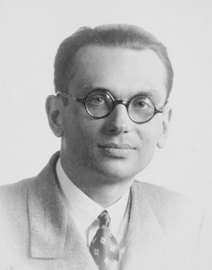
\includegraphics[height=5cm]{images/Goedel.jpg}

\LARGE
Gödel
\end{center}}

\begin{frame}\frametitle{Zwischenstand}

Wir haben bisher zwei Dinge erkannt:
\begin{enumerate}[(1)]
\item \alert{Prädikatenlogik ist sehr ausdrucksstark:}
mit ihr können wir z.B. das mathematische Konzept der Gleichheit axiomatisieren oder
Probleme über formale Sprachen beschreiben
\item \alert{Prädikatenlogisches Schließen ist unentscheidbar:}
man kann Probleme definieren, die nicht mehr algorithmisch lösbar sind
\end{enumerate}

Eignet sich Prädikatenlogik also als universelle Beschreibungssprache für
die Mathematik (und darüber hinaus)?
\bigskip

Dazu hat Kurt Gödel (1906--1978) einiges zu sagen \ldots

\end{frame}

\begin{frame}\frametitle{Gödels Einsichten}

Gödel zeigte einige wesentliche Dinge:
\begin{enumerate}[(1)]
\item \alert{Gödelscher Vollständigkeitssatz (1930):}\\
"`Es gibt ein konsistentes Verfahren, das alle Konsequenzen einer prädikatenlogischen Theorie
effektiv beweisen kann."'
\begin{itemize}
\item Alle wahren Sätze können endlich bewiesen werden
\item Prädikatenlogisches Schließen ist semi-entscheidbar
\end{itemize}\pause
%
\item \alert{1. Gödelscher Unvollständigkeitssatz (1931):} \\
"`Es gibt kein konsistentes Verfahren, das alle Konsequenzen der elementaren Arithmetik
effektiv beweisen kann."'
\begin{itemize}
\item Für jedes Verfahren gibt es Sätze über elementare arithmetische Zusammenhänge, die weder bewiesen noch
widerlegt werden können
\item Die Wahrheit elementarer arithmetischer Zusammenhänge ist nicht semi-entscheidbar
\end{itemize}\pause
\item \alert{2. Gödelscher Unvollständigkeitssatz (1931):} später
\end{enumerate}

Mehr dazu in späteren Vorlesungen \ldots

\end{frame}

% Entailment
% - Probleme, Reduktionen
% - Unentscheidbarkeit
% Model Checking
% - PSpace-Completeness
% Equality
% - Simulation (sat. preservation)
% Function symbols
% - Simulation (sat. preservation)



\begin{frame}\frametitle{Zusammenfassung und Ausblick}

Logisches Schließen ist ein Kernproblem der Prädikatenlogik;\\
es entspricht verschiedenen konkreten Fragen (Folgerung, Erfüllbarkeit, Allgemeingültigkeit)
\bigskip

Logisches Schließen über logischen Aussagem mit Gleichheit kann
auf logisches Schließen ohne Gleichheit reduziert werden\bigskip

Logisches Schließen in Prädikatenlogik ist unentscheidbar (gezeigt)
aber semi-entscheidbar (noch zu zeigen)

\anybox{yellow}{
Was erwartet uns als nächstes?
\begin{itemize}
\item Ein konkretes Verfahren zum logischen Schließen
\item Logik über endlichen Modellen und ihre praktische Anwendung
\item Gödels Unvollständigkeitssätze
\end{itemize}
}

\end{frame}




\begin{frame}[t]\frametitle{Bildrechte}

Folie \ref{frame_logiker}: (von oben)
\begin{itemize}
\item Aristoteles-Büste, römische Kopie, nach einer Skulptur des Bildhauers Lysippos, gemeinfrei
\item Gemälde von Johann Friedrich Wentzel d. Ä. (Ausschnitt), um 1700, gemeinfrei
\item Fotografie von 1912, gemeinfrei
\item Fotografie, um 1924, gemeinfrei
\end{itemize}
Folie \ref{frame_goedel}: Fotografie um 1926, gemeinfrei

\end{frame}


\end{document}